\begin{surferPage}[無次曲面(15個尖點)]{帶有15個尖點的五次曲面}
這個五次曲面具有15個$A_2$型奇異點(稱為尖點)。2005年奧利弗·萊布斯(Oliver Labs)在一篇文章中給出了此五次曲面以及相關的一系列曲面。15個尖點中的五個看起來會跟其他10個不同。實際上這五個尖點是$A_2^{++}$型,
而另外十個尖點是$A_2^{+-}$型的(更多資訊參見本圖冊裡面的簡單奇異點):
     \vspace*{-0.3em}
    \begin{center}
      \begin{tabular}{c@{\qquad}c}
        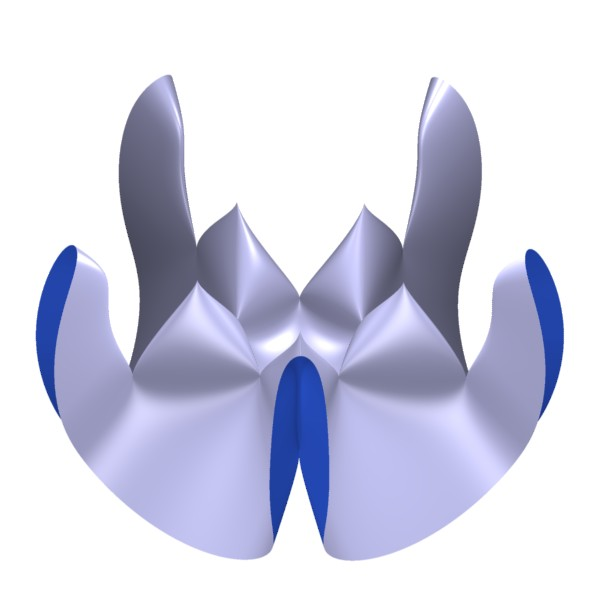
\includegraphics[height=1.2cm]{dessins_quint_15a2}
        &
        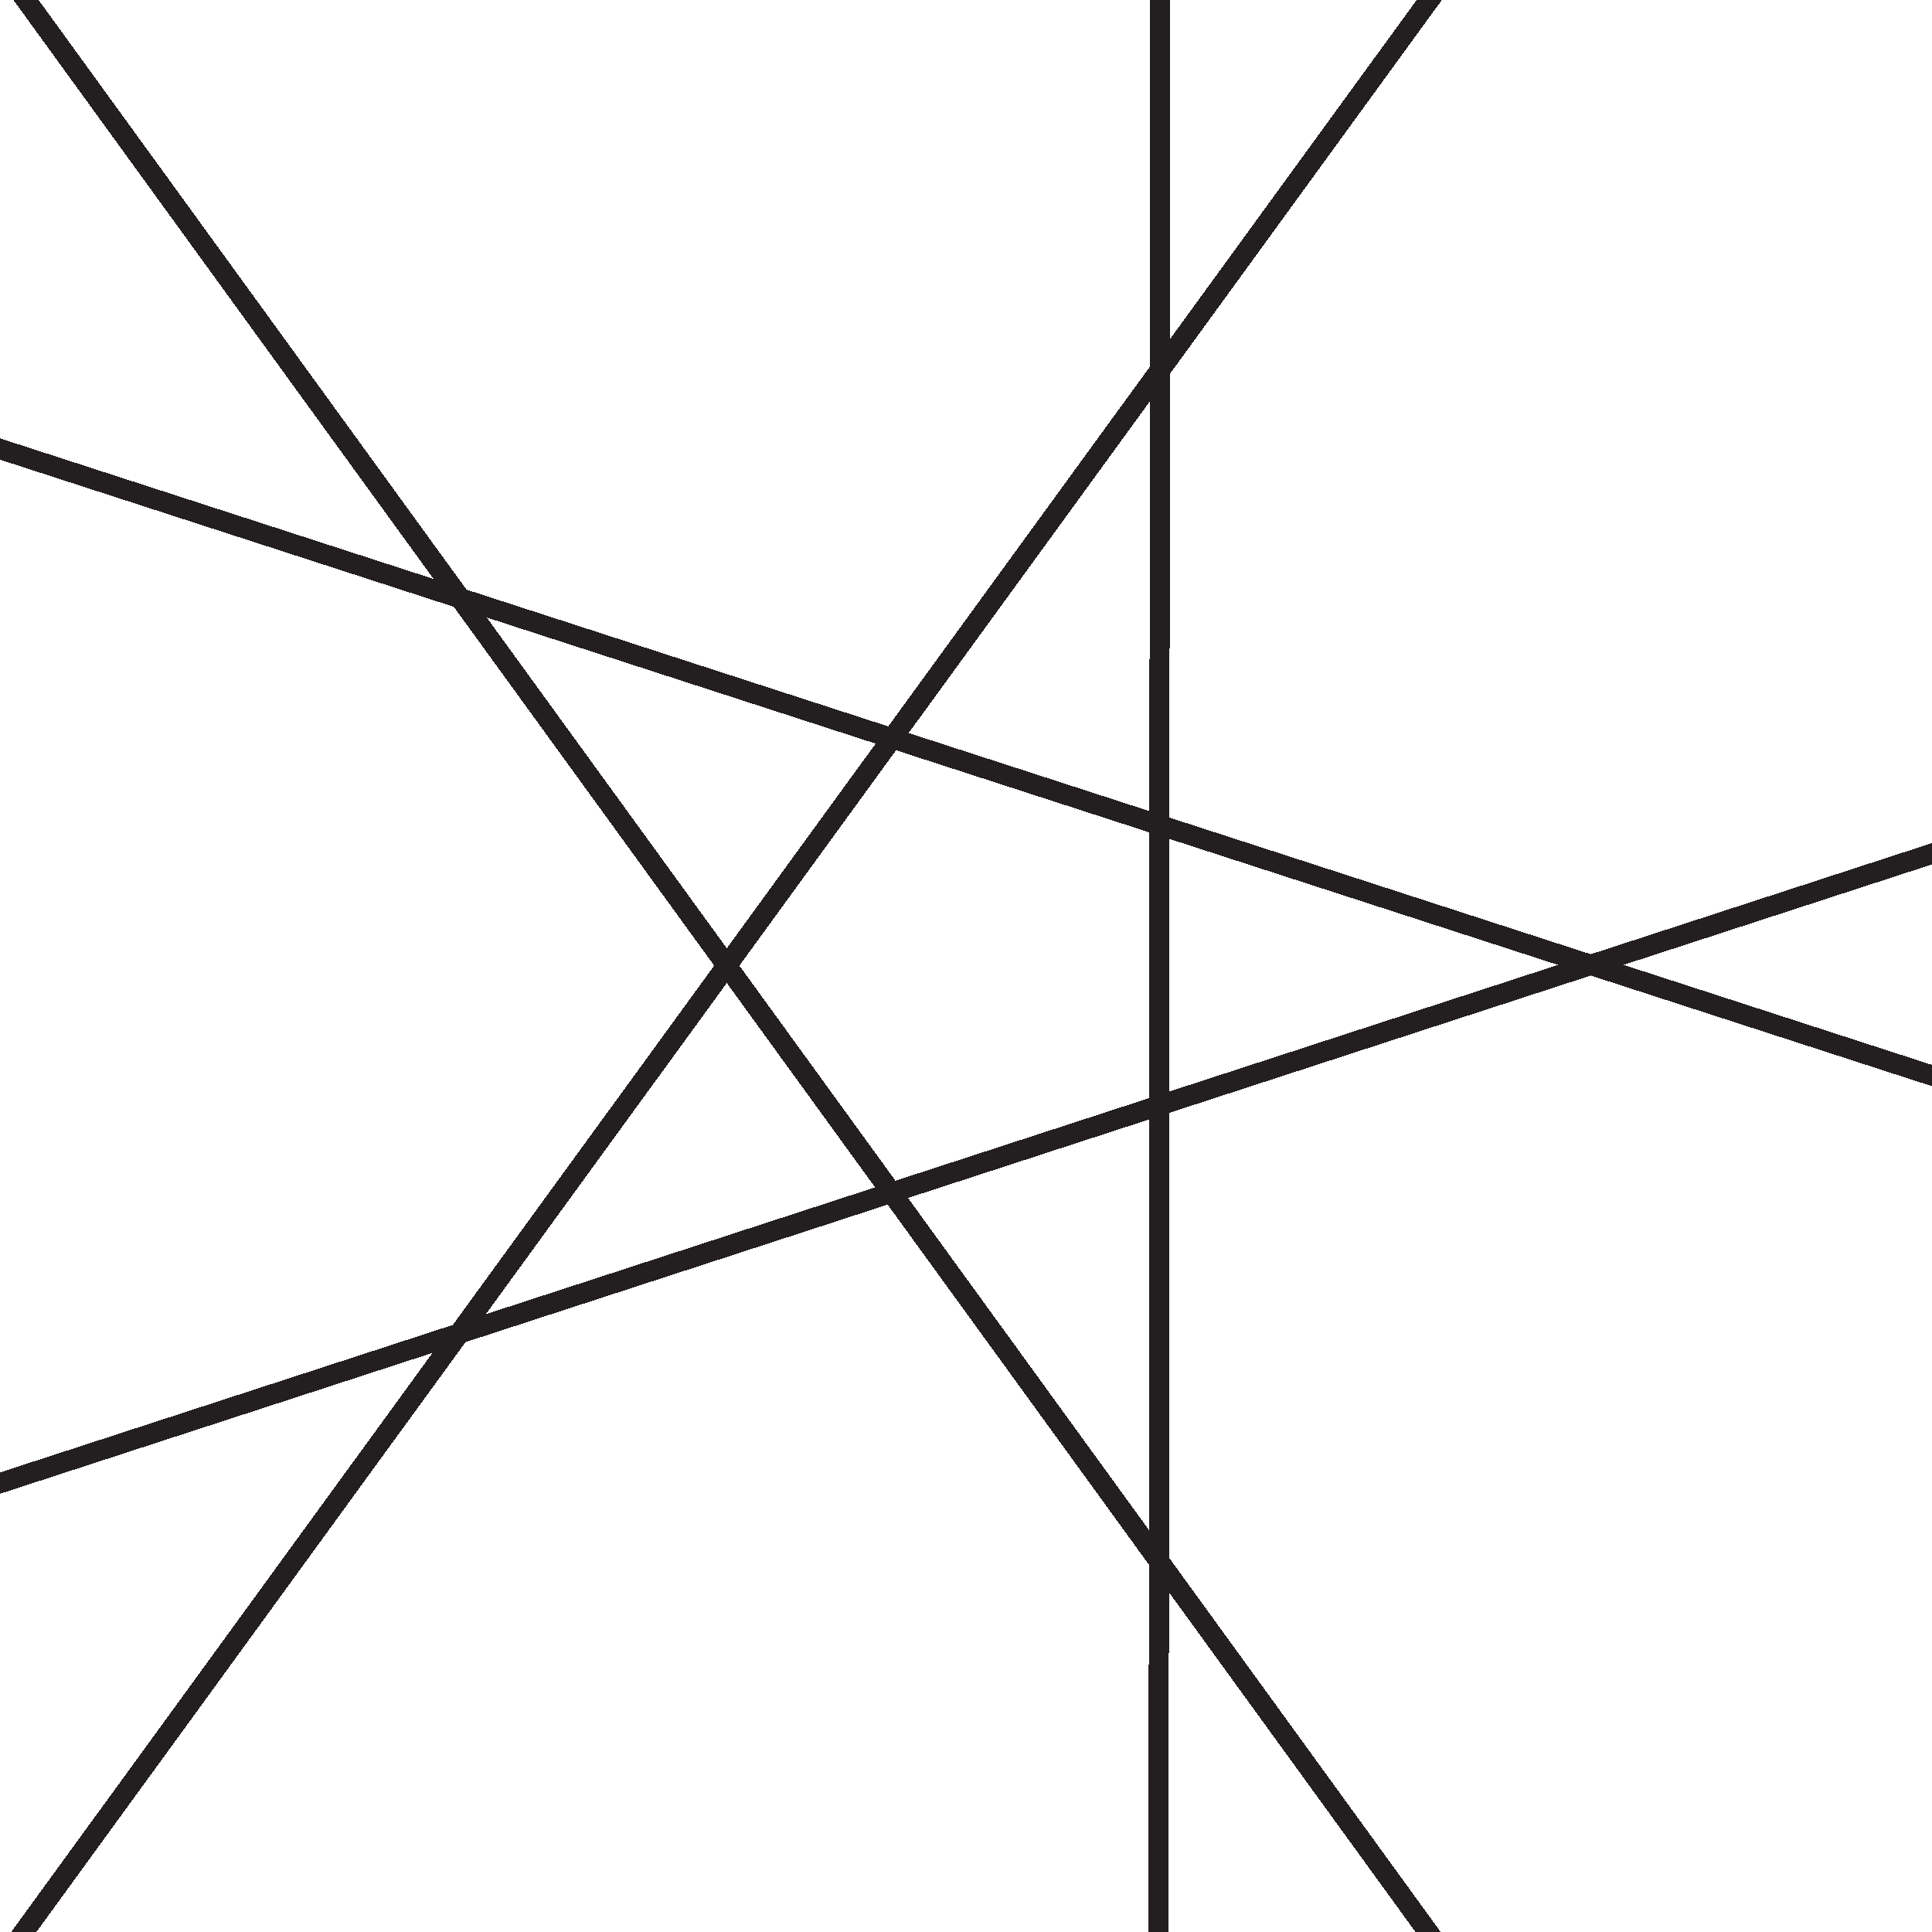
\includegraphics[height=1.2cm]{rp5.pdf}
      \end{tabular}
    \end{center}
    \vspace*{-0.3em}

此曲面具有方程$S_5(x,y) + t(z)=0,$其中$S_5(x,y)$為正五邊形(右圖),$t(z)$是我們曾多次提起的切比雪夫多項式(Tchebychev polynomial)的一種變形。
另外一種五次曲面(左圖)由沃爾夫巴斯構造出來。從中間圖可以看出,它和克勒佈施立方體(右圖)相關。
    \vspace*{-0.3em}
    \begin{center}
      \begin{tabular}{c@{\quad}c@{\quad}c}
        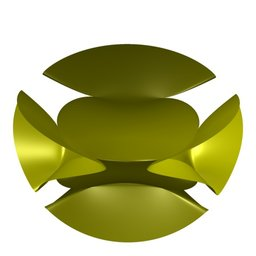
\includegraphics[height=1.2cm]{barthquintic_green}
        &
        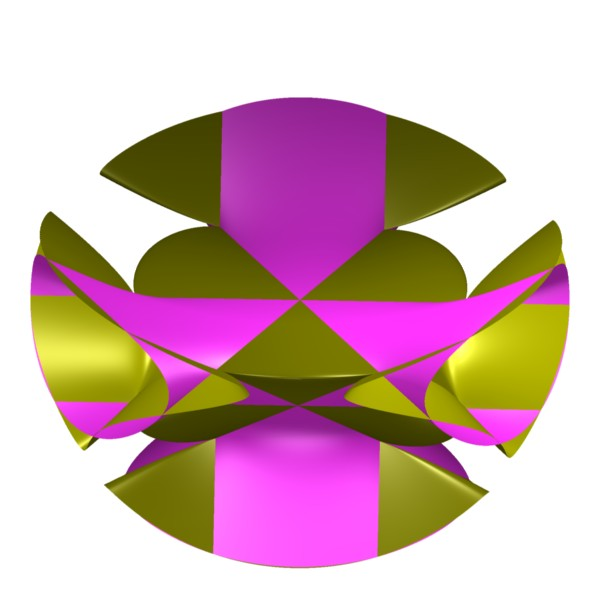
\includegraphics[height=1.2cm]{barthquintic_clebschcubic}
        &
        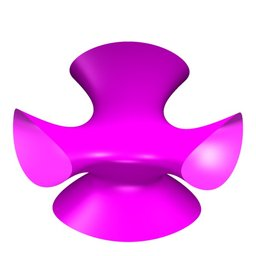
\includegraphics[height=1.2cm]{clebschcubic_pink}
      \end{tabular}
    \end{center}
    \vspace*{-0.3em}
\end{surferPage}
